\section{Perancangan Kapal}
\label{sec:perancangan-kapal}

\subsection{Sejarah Singkat Perancangan Kapal}
\label{subsec:sejarah-singkat-deskap}

Pada masa lalu, perancangan kapal lebih bergantung kepada pengalaman dan intuisi dari seorang insinyur perancang kapal daripada metode sains. Desainer menggunakan pendekatan heuristik dan \emph{trial-and-error} selama bertahun-tahun. Kemudian dengan perkembangan teknologi dan ilmu pengetahuan, metode ini secara perlahan digantikan dengan metode semi-empiris dan berdasarkan data statistik kapal-kapal yang sudah dibangun.

Pada masa ini, perancangan kapal adalah proses yang kompleks. Merancang kapal berarti mampu melihat kapal sebagai sebuah integrasi dari berbagai macam subsistem, seperti penanganan muatan, propulsi kapal dan akomodasi awak. Pendekatan desain modern mempertimbangkan seluruh siklus hidup kapal, dari konsep dan pembangunan hingga saat operasi dan kapal di-\emph{scrap} \citep{Papanikolaou_2014}. Pendekatan holistik ini bertujuan untuk mengoptimalkan kinerja kapal sepanjang siklus hidupnya, dengan mempertimbangkan berbagai faktor dan batasan.

Desain kapal melibatkan masalah optimasi yang kompleks, menyeimbangkan persyaratan yang bertentangan dari berbagai pemangku kepentingan seperti pemilik kapal, pembangun, dan regulator. Desain harus mencapai biaya konstruksi rendah, kapasitas angkut tinggi, efisiensi operasional, keselamatan, perlindungan lingkungan, dan faktor lainnya. Persyaratan desain awal merupakan hasil dari negosiasi dan kompromi di antara pengambil keputusan yang berpengalaman.

\subsection{Tahapan Utama Perancangan Kapal}
\label{subsec:tahapan-utama-deskap}

Secara tradisional, perancangan kapal dapat dibagi menjadi empat tahap utama yaitu:
\begin{enumerate}[label=\alph*.]
    \item \emph{Concept design}
    \item \emph{Preliminary design}
    \item \emph{Contract design}
    \item \emph{Detailed design}
\end{enumerate}

Dua tahap pertama juga dikenal dengan \emph{basic design}. Gambar \ref{fig:tahap-deskap} menunjukkan tahapan-tahapan pernacngan kapal yang bertujuan untuk mempertemukan antara tujuan khusus dari kapal tersebut ,menjadi sebuah fungsi tertentu, bentuk, volume, berat, performa teknis dan karakteristik ekonomi dari kapal yang dirancang.

\begin{figure}[ht]
  \centering
  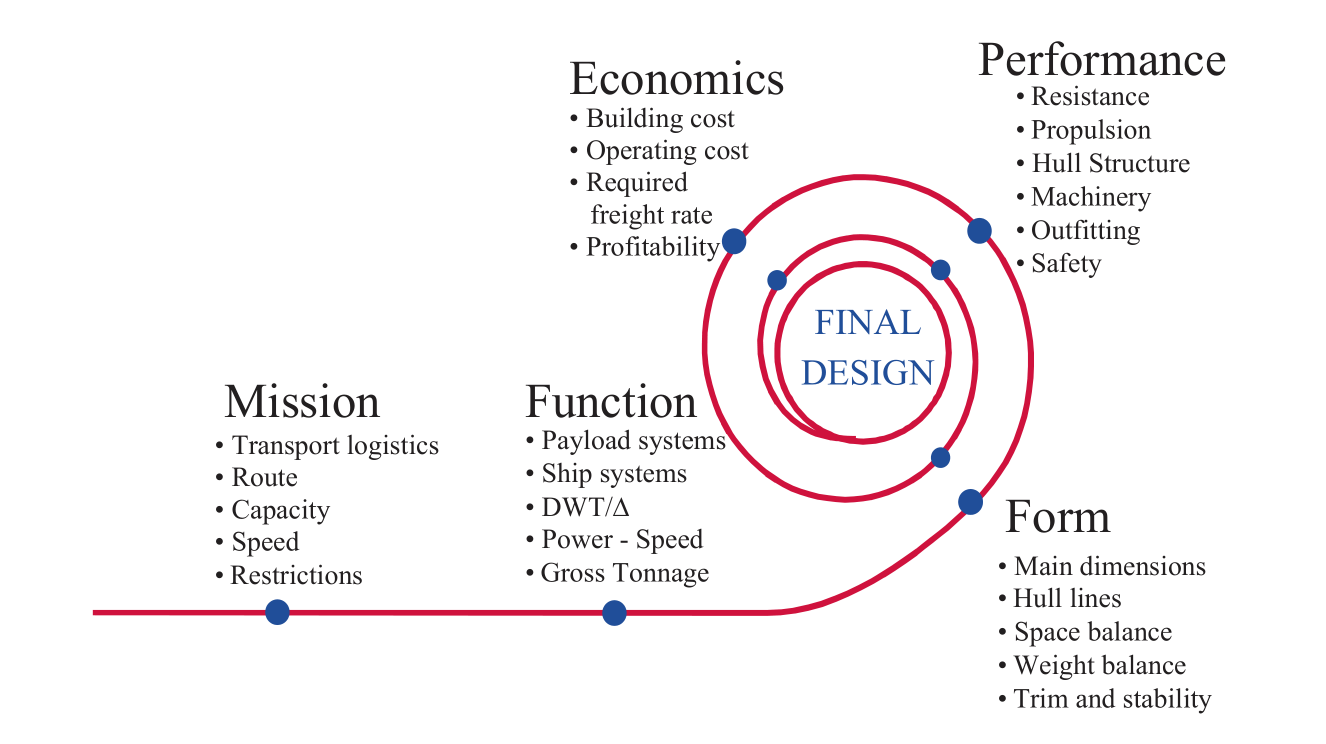
\includegraphics[width=0.95\textwidth,keepaspectratio]{gambar/ship design procedure.png}
  \caption{Proses Perancangan Kapal \citep{Levander_2003}.}
  \label{fig:tahap-deskap}
\end{figure}

\emph{Preliminary design} adalah tahapan desain dimana persyaratan atau spesifikasi yang diinginkan oleh pemilik kapal diterjemahkan menjadi karakteristik ekonomi dan karakteristik teknis dari kapal dengan metode optimasi. Optimasi disini bertujuan untuk menentukan biaya pembangunan kapal tersebut agar semakin kecil atau dalam operasionalnya nanti yang paling menguntungkan.
    

\subsection{Tujuan dari \emph{Preliminary Design}}
\label{subsec:tujuan-desain-awal}

\emph{Preliminary design} atau Desain kapal awal mencakup tujuan-tujuan yang lebih rinci berikut ini:

\begin{enumerate}[label=\textbullet]
    \item Pemilihan dimensi utama kapal
    \item Pengembangan bentuk lambung kapal (bagian terendam dan bagian di atas air)
    \item Spesifikasi jenis dan ukuran mesin utama serta sistem propulsi (penggerak)
    \item Perkiraan jenis dan daya mesin bantu
    \item Desain tata letak umum ruang utama dan ruang bantu (ruang kargo, ruang mesin, dan akomodasi)
    \item Spesifikasi peralatan penanganan kargo
    \item Desain elemen struktural utama untuk kekuatan longitudinal dan transversal
    \item Pengendalian kemampuan mengapung, stabilitas, trim, dan freeboard (regulasi stabilitas dan garis muat)
    \item Pengukuran tonase (GT)
\end{enumerate}

Harus Dipahami bahwa penentuan semua elemen desain kapal di atas harus mematuhi spesifikasi berbagai aturan dan peraturan maritim nasional dan internasional, yang diberlakukan oleh otoritas nasional dan internasional (negara bendera dan negara pelabuhan, IMO) atau oleh lembaga klasifikasi internasional yang diakui. Dalam kasus kekurangan spesifikasi regulasi, dipahami bahwa kapal yang dirancang dan dibangun harus sesuai dengan keadaan terkini dalam ilmu dan teknologi pembuatan kapal.

Desain kapal awal adalah studi kelayakan tekno-ekonomi, yang berfokus pada kapal sebagai elemen kunci dalam sistem transportasi maritim global. Proses ini melibatkan pertimbangan perkembangan terbaru dalam teknologi pembuatan kapal dan kelautan, serta persyaratan fisik, teknis, dan ekonomi dari pemilik kapal, serta mematuhi peraturan nasional dan internasional.

Kompleksitas desain kapal muncul dari kebutuhan untuk menyeimbangkan berbagai persyaratan dan peraturan keselamatan yang sering kali bertentangan. Kondisi operasi unik kapal, termasuk interaksinya dengan air dan udara, dan beban dinamis yang dari kapal itu sendiri dan muatan yang diangkut  menghadirkan tantangan ilmiah dan teknologi yang unik.

\begin{figure}[ht]
  \centering
  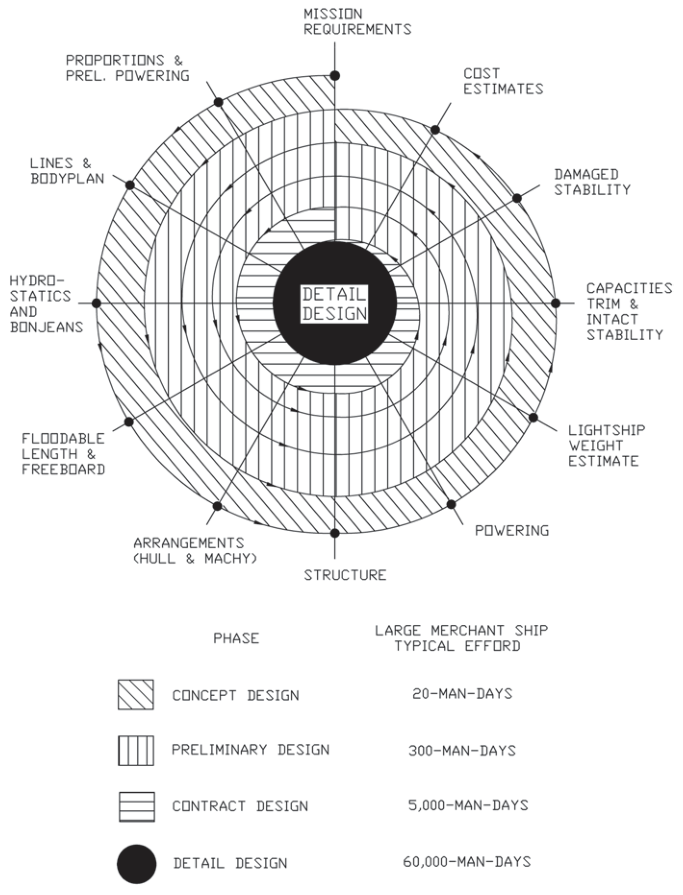
\includegraphics[width=0.75\textwidth,keepaspectratio]{gambar/design-spiral.png}
  \caption{Proses Desain Spiral \citep{Taggart_1980}.}
  \label{fig:design-spiral}
\end{figure}

Desain kapal sering kali melampaui teknologi dan sains murni, menggabungkan elemen seni, terutama dalam desain jenis kapal tertentu seperti kapal pesiar penumpang dan yacht. Banyak masalah desain diselesaikan menggunakan intuisi dan pengalaman arsitek kapal daripada hanya mengandalkan alat dukungan keputusan modern, terutama karena keterbatasan waktu dan kompleksitas masalah \citep{Papanikolaou_2014}. Meskipun demikian, kemajuan terbaru dalam teknologi informasi membuat adaptasi insinyur baru lebih mudah kedalam seluruh tahapan perancangan kapal.


\subsection{Prosedur Perancangan Kapal}
\label{prosedural-deskap}

Prosedur atau pola pikir yang biasa digunakan dalam perancangan kapal adalah desain spiral. Dikatakan desain spiral karena proses desain antar tahapan maupun bagiannya harus dilakukan dengan urut dan saling bertimbal balik. Ketikan ada persyaratan yang tidak dapat dipenuhi pada suatu tahapan desain baik dari sisi spesifikasi yang diinginkan pemilik kapal maupun regulator, dilakukan evaluasi pada proses sebelumnya sehingga dikatakan desain spiral.


Spiral desain secara efektif menggambarkan urutan proses desain kapal melalui berbagai langkah desain, prosedur iteratif yang berulang untuk penentuan dimensi kapal dan sifat-sifat lainnya, dan akhirnya, pendekatan bertahap menuju tahap akhir desain kapal yang detail. Dalam gambar \ref{fig:design-spiral}, diberikan beberapa standar atau beban dalam hari kerja untuk penyelesaian setiap tahap desain kapal, grafik tersebut disesuaikan proses desain kapal niaga besar pada akhir 1950-an.


% \subimport{2-ros2}{1-ros2-node.tex}
% \subimport{2-ros2}{2-rmw.tex}
% \subimport{2-ros2}{3-rcl.tex}
% \subimport{2-ros2}{4-ros2-interface.tex}
% \subimport{2-ros2}{5-ros2-cli.tex}
% \subimport{2-ros2}{6-rqt.tex}
% \subimport{2-ros2}{7-rviz2.tex}
